\documentclass[12pt]{article}
\usepackage{fancyhdr}
\usepackage{lastpage}
\usepackage{geometry}
\usepackage{amsmath}
\usepackage{setspace}
\usepackage{graphicx}
\usepackage{caption}
\geometry{a4paper,scale=0.8}
\pagestyle{plain}
\renewcommand{\headrulewidth}{0.4pt}
\renewcommand{\footrulewidth}{0.4pt}
\setlength{\baselineskip}{23pt}


\begin{document}
	\thispagestyle{plain}
	\noindent \Large \textbf{Multi-Factor stock pitching model using ML}\\ \\
	\noindent Fu, Sun, Wang BY, Wang PY and Zhuang (2019)\\
	\noindent \normalsize \textit{Singapore Management University, Singapore}\\ \\
	\noindent July 2019
	
\section{Abstract} % Numbered section
This paper applied a machine learning method of support vector machine(SVM) to stock pitching process. Given the information of eligible stocks listed in the Chinese stock market during the period of January 2009 to May 2019, we attempt to utilize SVM to construct a portfolio consist of 100 stocks with the highest potential returns. In order to evaluate the efficiency, the SVM model is compared with stochastic gradient descent(SGD). The indicators lead to a conclusion that SVM outperforms SGD and achieves a total return of 800\% in the time period of 2009 to 2019.

	
\section{Introduction} % Numbered section
Technics for stock prediction is updating as the advancement in artificial intelligence.  One of the biggest problems of existing stock price prediction models is that linear models fail to capture the randomness in the financial time series data. Therefore, we introduce machine learning methods to interpret the non-linear trend. Multiple machine learning methods have been applied in the financial time series analysis field. Among those methods, support vector machine(SVM) works well when used to solve non-linear regression or classification problems. The maximum-margin hyperplane in the SVM model represents the largest separation between the two classes. SVMs are based on the structural risk minimization principle which allows them to estimate a function by minimizing an upper bound of generalization error.\cite{Vapnik} That's why we introduce the support vector machine(SVM) in this case.\\

The main objective of this paper is to train an SVM model and use it to construct a portfolio consist of 100 stocks. In the stock selection process, we used monthly data from January 2009 to May 2019, 125 sets of data in total,  and based multi-factor model on selected 70 factors. To evaluate the efficiency of the SVM method, we constructed another portfolio under the framework of stochastic gradient descent(SGD). We compare the two portfolio performance and the results show clearly that the SVM model performed better. The remainder of the paper is constructed as follows. Section 2 introduces the data of the model, including the process of pre-processing data. Section 3 gives a brief introduction to the methodology as well as the research design. In Section 4, we discussed the backtest results, comparing SVM with SGD method and quantify the results by testing on the net asset value(NAV), excess volatility and information ratio.\\
		
\section{Data}
text..


\section{Methodology \& Research Design}
text..

\newpage
\section{Backtest Results}

In this section, we construct a simple investment strategy based on the previous SVM or SGD model's prediction. The logic of this strategy can be stated as: we select 100 stocks with the highest possibility of positive return in the following month under SVM model prediction and adopted a equal weight among all the stocks. The Net Asset Value (NAV) of the portfolio can be visualized as the cumulative excess return line in the figure below.\\ \\

\noindent And we evaluate each portfolio's performance based on three indicators:
	\begin{itemize}
		\item Annual excess return: Calculated by $12*\mu$, where $\mu$ is the average excess return of one year.
		\item Anuual excess volatility: Calculated by $\sqrt{12 * \sigma^2}$, where $\sigma^2$ is the annual variance of whole year excess return 
		\item Information Ratio (IR): Calculated by $\frac{\textnormal{Anuual excess return}}{\textnormal{Annual excess volatility}}$ , and it can be translated as the premium for portfolio taking each unit of active risk. So the bigger IR is, the better portfolio perform.
	\end{itemize}

\begin{figure}[h]
	\centering
	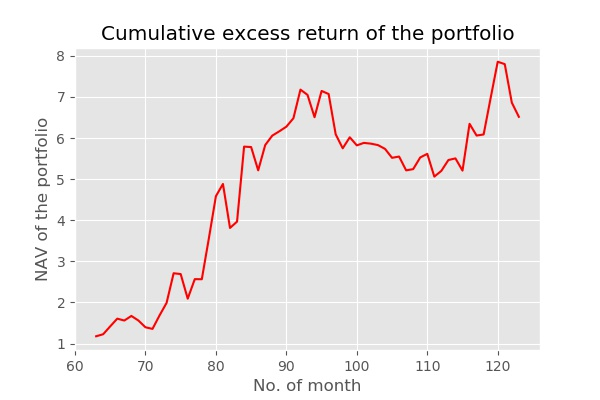
\includegraphics[width=0.6\linewidth]{pic//NAV_SVM.jpg}
	\caption*{Figure 01: Portfolio based on SVM}
	\label{fig:label}
\end{figure}

\begin{figure}[h]
	\centering
	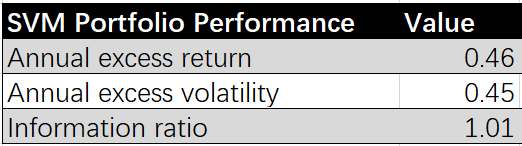
\includegraphics[width=0.6\linewidth]{pic//SVM_Performance.png}
	\caption*{Table 01: SVM Portfolio performance}
	\label{fig:label}
\end{figure}
\newpage
\begin{figure}[h]
\centering
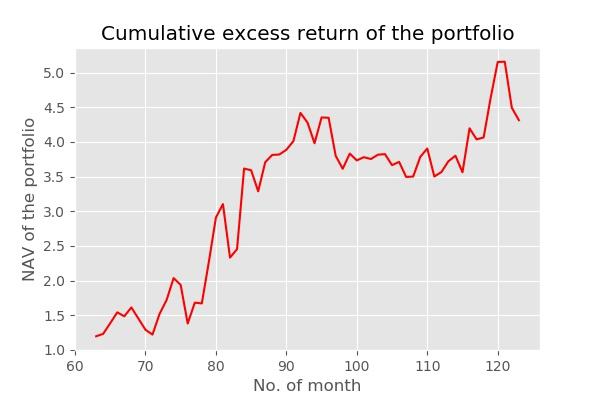
\includegraphics[width=0.6\linewidth]{pic//NAV_SGD.jpg}
\caption*{Figure 02: Portfolio based on SGD}
\label{fig:label}
\end{figure}

\begin{figure}[h]
	\centering
	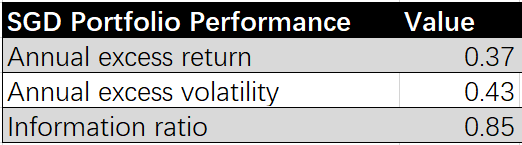
\includegraphics[width=0.6\linewidth]{pic//SGD_Performance.png}
	\caption*{Table 02: SGD Portfolio performance}
	\label{fig:label}
\end{figure}



\section{Conclusion} % Numbered section

text..

\begin{thebibliography}{999}
	
	\bibitem{Vapnik}
	Vapnik, V. N., \& Vapnik, V. ,
	\emph{Statistical learning theory
		(Vol. 1). }.
	New York,
	1998.
	
\end{thebibliography}

\end{document}
